\title{simulations}

In this section we shall take a look at the simulations for the cartesian stabilization in matlab.
The simulations are done with the following values.
\begin{equation}
(x_{ref},y_{ref},\theta_{ref})=(100,100,\frac{\pi}{2})\\
k_{s}=[0.1,0.2,0.6,0.7]\\
k_{\theta}=0.3
\end{equation}

\begin{figure} 
\centering
 	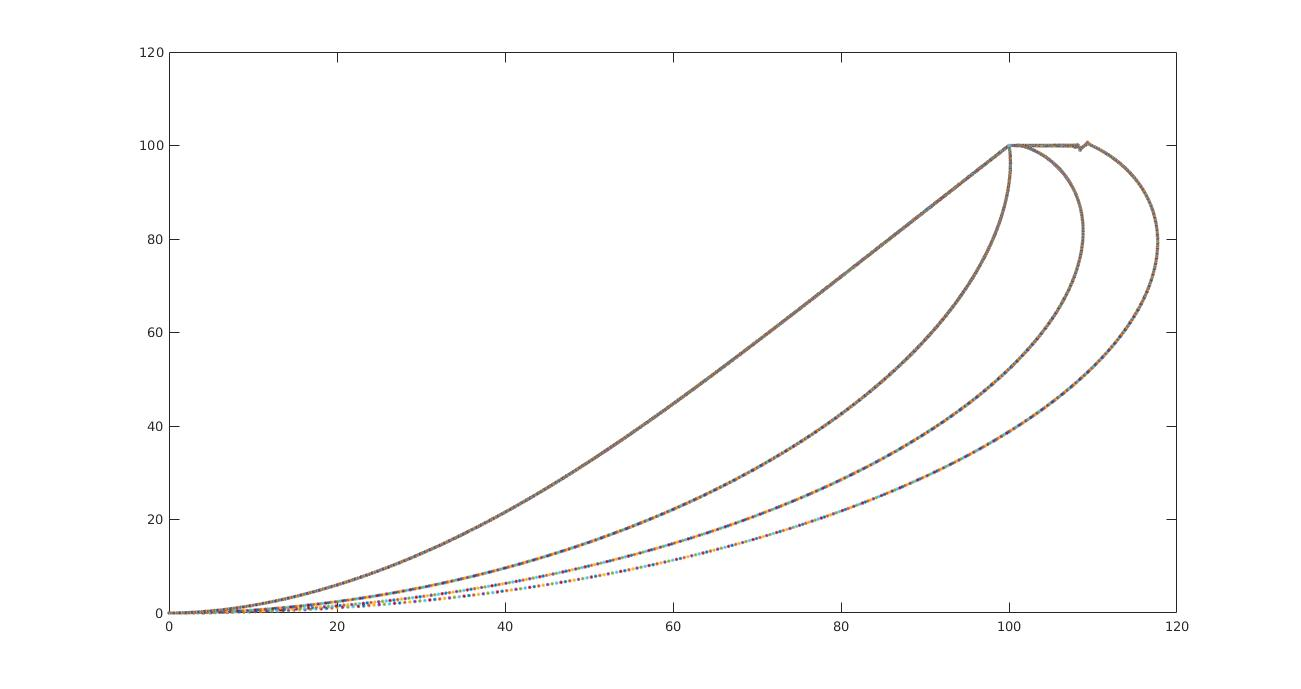
\includegraphics[width=1\textwidth]{figures/xycartplot.jpg}
	
	
	\caption{x y plot} 
 	\label{fig:xyplot} 
\end{figure}

\begin{figure} 
\centering
 	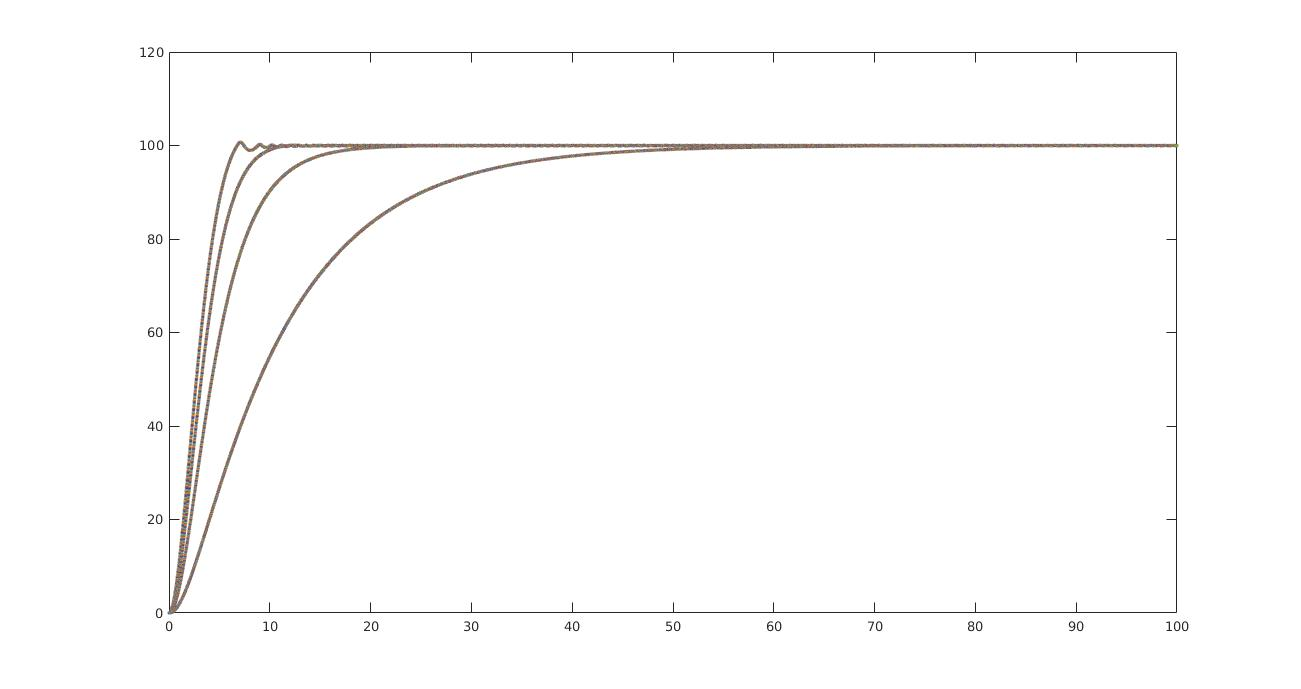
\includegraphics[width=1\textwidth]{figures/yvstime.jpg}
	
	
	\caption{Y and time} 
 	\label{fig:yvstime} 
\end{figure}

\begin{figure} 
\centering
 	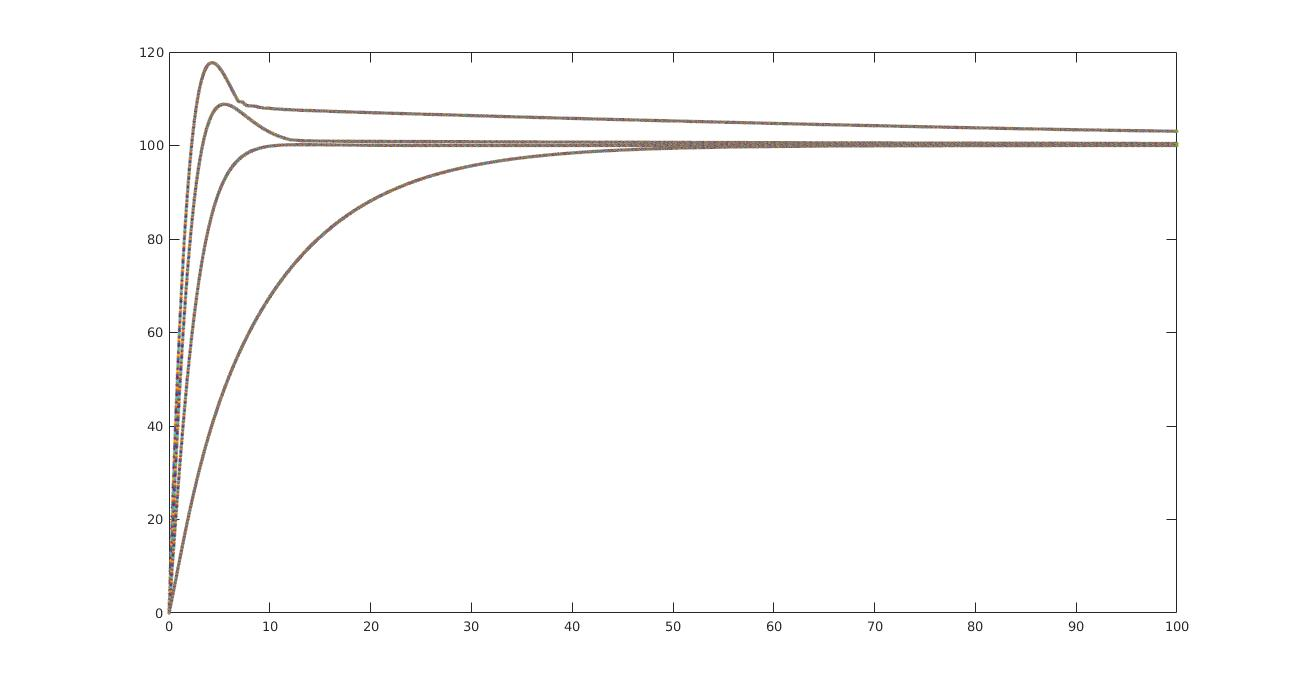
\includegraphics[width=1\textwidth]{figures/xvstime.jpg}
	
	
	\caption{X and time} 
 	\label{fig:xvstime} 
\end{figure}

By closer examination we can see that the system is stabel only if the local stability conditions are satisfied. For example $k_{\theta}$>$k_{s}$>0